\documentclass[12pt, a4paper, reqno]{article}
\usepackage[utf8]{inputenc}
\usepackage{amsmath, amsfonts, amssymb, amsthm, graphicx}
\usepackage[ruled]{algorithm2e}
\usepackage{caption}

\usepackage{hyperref}
\usepackage[dvipsnames]{xcolor}
\hypersetup{colorlinks, linkcolor={MidnightBlue}, citecolor={MidnightBlue}, urlcolor={MidnightBlue}} 

\usepackage{tikz}


\numberwithin{equation}{section}
\parindent 0mm
\addtolength{\textwidth}{2 truecm}
\setlength{\hoffset}{-1 truecm}

\newtheorem*{theorem*}{Theorem}
\newtheorem*{cor*}{Corollary}

\newcommand{\norm}[1]{\left\lVert#1\right\rVert}
\newcommand{\e}{\epsilon}
\newcommand{\w}{\omega}
\newcommand{\R}{\mathbb{R}}
\newcommand{\N}{\mathbb{N}}
\newcommand{\Q}{\mathbb{Q}}
\newcommand{\Z}{\mathbb{Z}}
\renewcommand{\ae}[1]{\text{ \hspace{5pt} a.e. #1}}

\begin{document}

\title{Combining $l^1$ Penalization with Higher Moment Feasible Sets in Regression Models: a STAT8053 Project}
\author{Austin David Brown}
\date{\today}
\maketitle

\section{Introduction}


In some sense we want a stable solution
So we can control the hieight and widths by using l norms
This is one way to enforce a stable solution

I want a "stable" solution
If the solution sucks at predicting, we can interpret this as the solution is not stable.

TODO

I asked a question during class as to what happens if you add higher moments to elasticnet. This project seeks to explore that question.


\begin{center}
\begin{minipage}{.5\textwidth}
  \centering
  \includegraphics[width=.9\linewidth]{elnet.pdf}
\end{minipage}%
\begin{minipage}{.5\textwidth}
  \centering
  \includegraphics[width=.9\linewidth]{4_moment.pdf}
\end{minipage}
\captionof{figure}{Elasticnet on the left and 4th moment with l1 on the right}
\end{center}

\begin{center}
\begin{minipage}{.5\textwidth}
  \centering
  \includegraphics[width=.9\linewidth]{elnet.pdf}
\end{minipage}%
\begin{minipage}{.5\textwidth}
  \centering
  \includegraphics[width=.9\linewidth]{1andinf.pdf}
\end{minipage}
\captionof{figure}{Elasticnet on the left and l1 and infinity norm on the right}
\end{center}





\section{Implementation}

TODO currently library is implemented assuming user knows what they are doing so it will crash. This can easily be updated but it saves time.

TODO talk about step sizes

TODO talk about convergence guarantee

The package can be found here \cite{pros}.
The goal was to make an package usable by scientists and researchers.
For speed, $C++$ was used along with the Eigen library \cite{eigen} for matrix computations. This is analogous to using Fortran with LAPACK.
To interact with R, 2 interfacing layers need to be created: an R to C interface and an R script that the user calls functions from.
The benefit is that any other language can then be interfaced with the library.
The following diagram illustrates the idea.

\vspace{.5cm}
\begin{tikzpicture}[level distance=8em, sibling distance=10em,
  every node/.style = {shape=rectangle, draw, align=center}]]
  \node {PROS C++ code}
    child { node {R to C Interface} 
      child { node {R Interface} }
    }
    child { node {Python Interface} 
      child { node {$\ldots$} }
    }
    child { node {MatLab Interface} 
      child { node {$\ldots$} }
    }
    child { node {Julia Interface} 
      child { node {$\ldots$} }
    };
\end{tikzpicture}
\captionof{figure}{TODO}
\vspace{.5cm}


In the glmnet paper \cite{glmnet}, they use coordinate descent.
With the elasticnet \cite{elasticnet} penalty, this results in a closed form coordiante-wise minimization soluton.

The l1 penalty is not differentiable, but it is separable meaning that it can be decomposed into a sum.

First, I wrote the entire program using Subgradient coordinate descent using guidelines from \cite{wright_cd_algs}.
The algorithm is

\[
L(\beta) = \frac{1}{2} \norm{y - X \beta}_2^2 + \lambda P(\beta)
\]

\vspace{.5cm}
\begin{algorithm}[H]
\caption{Subgradient Coordinate Method}
Choose $\beta^0 \in \R^p$, Choose the tolerance $\delta > 0$;

Set $k \gets 0$

\Repeat{Until the loss difference $\Delta L$ is less than $\delta$}{ 

  Set the step size $h^k > 0$

  Permute $I = \{1, \ldots, p\}$

  \For {$i \in I$}{

    $\beta^{k + 1}_i \gets \beta^{k}_i - h^i g^i$ where $g^i \in (\partial L)_i$

  }

  $k \gets k + 1$
}

\end{algorithm}
\vspace{.5cm}


The subgradient makes this algorithm difficult in general.
The convergence is dependent on the step sizes, the algorithm is not a descent method.
Another issue is that we cannot do line search due to the subgradient.
The step sizes were chosen due to Nesterov \cite{nesterov} as diminishing with $\frac{R}{\sqrt{k + 1}}$.

The better algorithm is proximal gradient descent.
Because we constructed everything to be seperable the proximal mapping is done coordinate wise.
The algorithm is

\[
L(\beta) = \norm{y - X \beta}_2^2 + \lambda P(\beta)
\]

\vspace{.5cm}
\begin{algorithm}[H]
\caption{Proximal Gradient Coordinate Descent}
Choose $\beta^0 \in \R^p$, Choose the tolerance $\delta > 0$;

Set $k \gets 0$

\Repeat{Until the loss difference $\Delta L$ is less than $\delta$}{ 

  Set the step size $h^k > 0$

  Permute $I = \{1, \ldots, p\}$

  \For {$i \in I$}{

    $\beta^{k + 1}_i \gets (\textbf{prox}_{h^k L})_i ( \beta^k_i - h^k \langle X_i, y - X \beta \rangle )$

  }

  $k \gets k + 1$
}
\end{algorithm}
\vspace{.5cm}

The step size is chosen by diminishing step size, but I should do line search. This is easy to implement.

The cross validation was implemented with the warm starting algorithm.

\vspace{.5cm}
\begin{algorithm}[H]
\caption{Warm Start Cross-Validation}
TODO
\end{algorithm}
\vspace{.5cm}


%
% Bib
%
\begin{thebibliography}{1}

\bibitem{pros}
PROS. \href{https://github.com/austindavidbrown/pros}{github.com/austindavidbrown/pros}

\bibitem{boyd_proximalalgs}
Neal Parikh and Stephen Boyd. 2014. Proximal Algorithms. Found. Trends Optim. 1, 3 (January 2014), 127-239. DOI=10.1561/2400000003 http://dx.doi.org/10.1561/2400000003

\bibitem{wright_cd_algs}
Stephen J. Wright. 2015. Coordinate descent algorithms. Math. Program. 151, 1 (June 2015), 3-34. DOI=10.1007/s10107-015-0892-3 http://dx.doi.org/10.1007/s10107-015-0892-3

\bibitem{eigen}
Guennebaud, Gaël (2013). Eigen: A C++ linear algebra library (PDF). Eurographics/CGLibs.

\bibitem{glmnet}
Jerome Friedman, Trevor Hastie, Robert Tibshirani (2010). Regularization Paths for Generalized Linear Models via Coordinate Descent. Journal of Statistical Software, 33(1), 1-22. URL http://www.jstatsoft.org/v33/i01/.

\bibitem{elasticnet}
Zou, H. and Hastie, T. (2005). Regularization and variable selection via the elastic net. Journal of the Royal Statistical Society: Series B, 67, 301–320.

\bibitem{nesterov}
Yurii Nesterov. 2014. Introductory Lectures on Convex Optimization: A Basic Course (1 ed.). Springer Publishing Company, Incorporated.

\end{thebibliography}

\end{document}

